\documentclass{article}

% Required packages for algorithm environment
\usepackage{algorithm}
\usepackage{algorithmicx}
\usepackage{algpseudocode}
\usepackage{amsmath}
\usepackage{amssymb}
\usepackage{booktabs}
\usepackage{graphicx}

\title{IoMT Security: Post-Quantum Mutual Authentication}
\author{Your Name}
\date{\today}

\begin{document}

\maketitle

\section{Introduction}
Your introduction text here.

\section{Proposed Protocol}

\begin{algorithm}[h]
\caption{PQC-MFA Authentication Protocol}
\label{alg:pqc-mfa}
\begin{algorithmic}[1]
\State \textbf{Patient (P) Initialization:}
\State Generate fresh nonce $N_p$ and identity $ID$
\State \textbf{Step 1:} $P \rightarrow S$: Send $(ID, N_p)$
\State
\State \textbf{Server (S) Processing:}
\State Receive $(ID, N_p)$ from Patient
\State Generate fresh nonce $N_s$ and session key $K_{session}$
\State Compute $H = hash(K_{session})$
\State Sign hash: $\sigma = Sign_{sk(S)}(H)$
\State \textbf{Step 2:} $S \rightarrow P$: Send $(N_s, \sigma)$
\State
\State \textbf{Patient Verification:}
\State Receive $(N_s, \sigma)$ from Server
\State Verify signature using $pk(S)$
\State Extract session key $K_{session}$
\State \textbf{Output:} Authenticated session established
\end{algorithmic}
\end{algorithm}

\section{Security Comparison}

% Include the security comparison table
\begin{table}[h]
\centering
\caption{Security Feature Comparison}
\label{tab:security_comparison}
\begin{tabular}{lcccc}
\toprule
\textbf{Attack Type} & \textbf{Xu et al. [1]} & \textbf{Chen et al. [3]} & \textbf{Kumar et al. [5]} & \textbf{Proposed PQC-MFA} \\
\midrule
Replay Attack & \checkmark & \checkmark & \checkmark & \checkmark \\
Man-in-the-Middle (MitM) & \checkmark & \checkmark & \checkmark & \checkmark \\
Impersonation & \checkmark & \checkmark & \checkmark & \checkmark \\
Quantum 'Harvest Now, Decrypt Later' & \times & \times & \checkmark\textsuperscript{*} & \checkmark \\
Forward Secrecy & \times & \times & \checkmark\textsuperscript{*} & \checkmark \\
Single Point of Failure (SPoF) & \checkmark & \checkmark & \checkmark\textsuperscript{*} & \checkmark \\
\bottomrule
\end{tabular}
\begin{flushleft}
\small
\textsuperscript{*} Requires hardware support
\end{flushleft}
\end{table}


\section{Performance Results}

\begin{figure}[h]
\centering
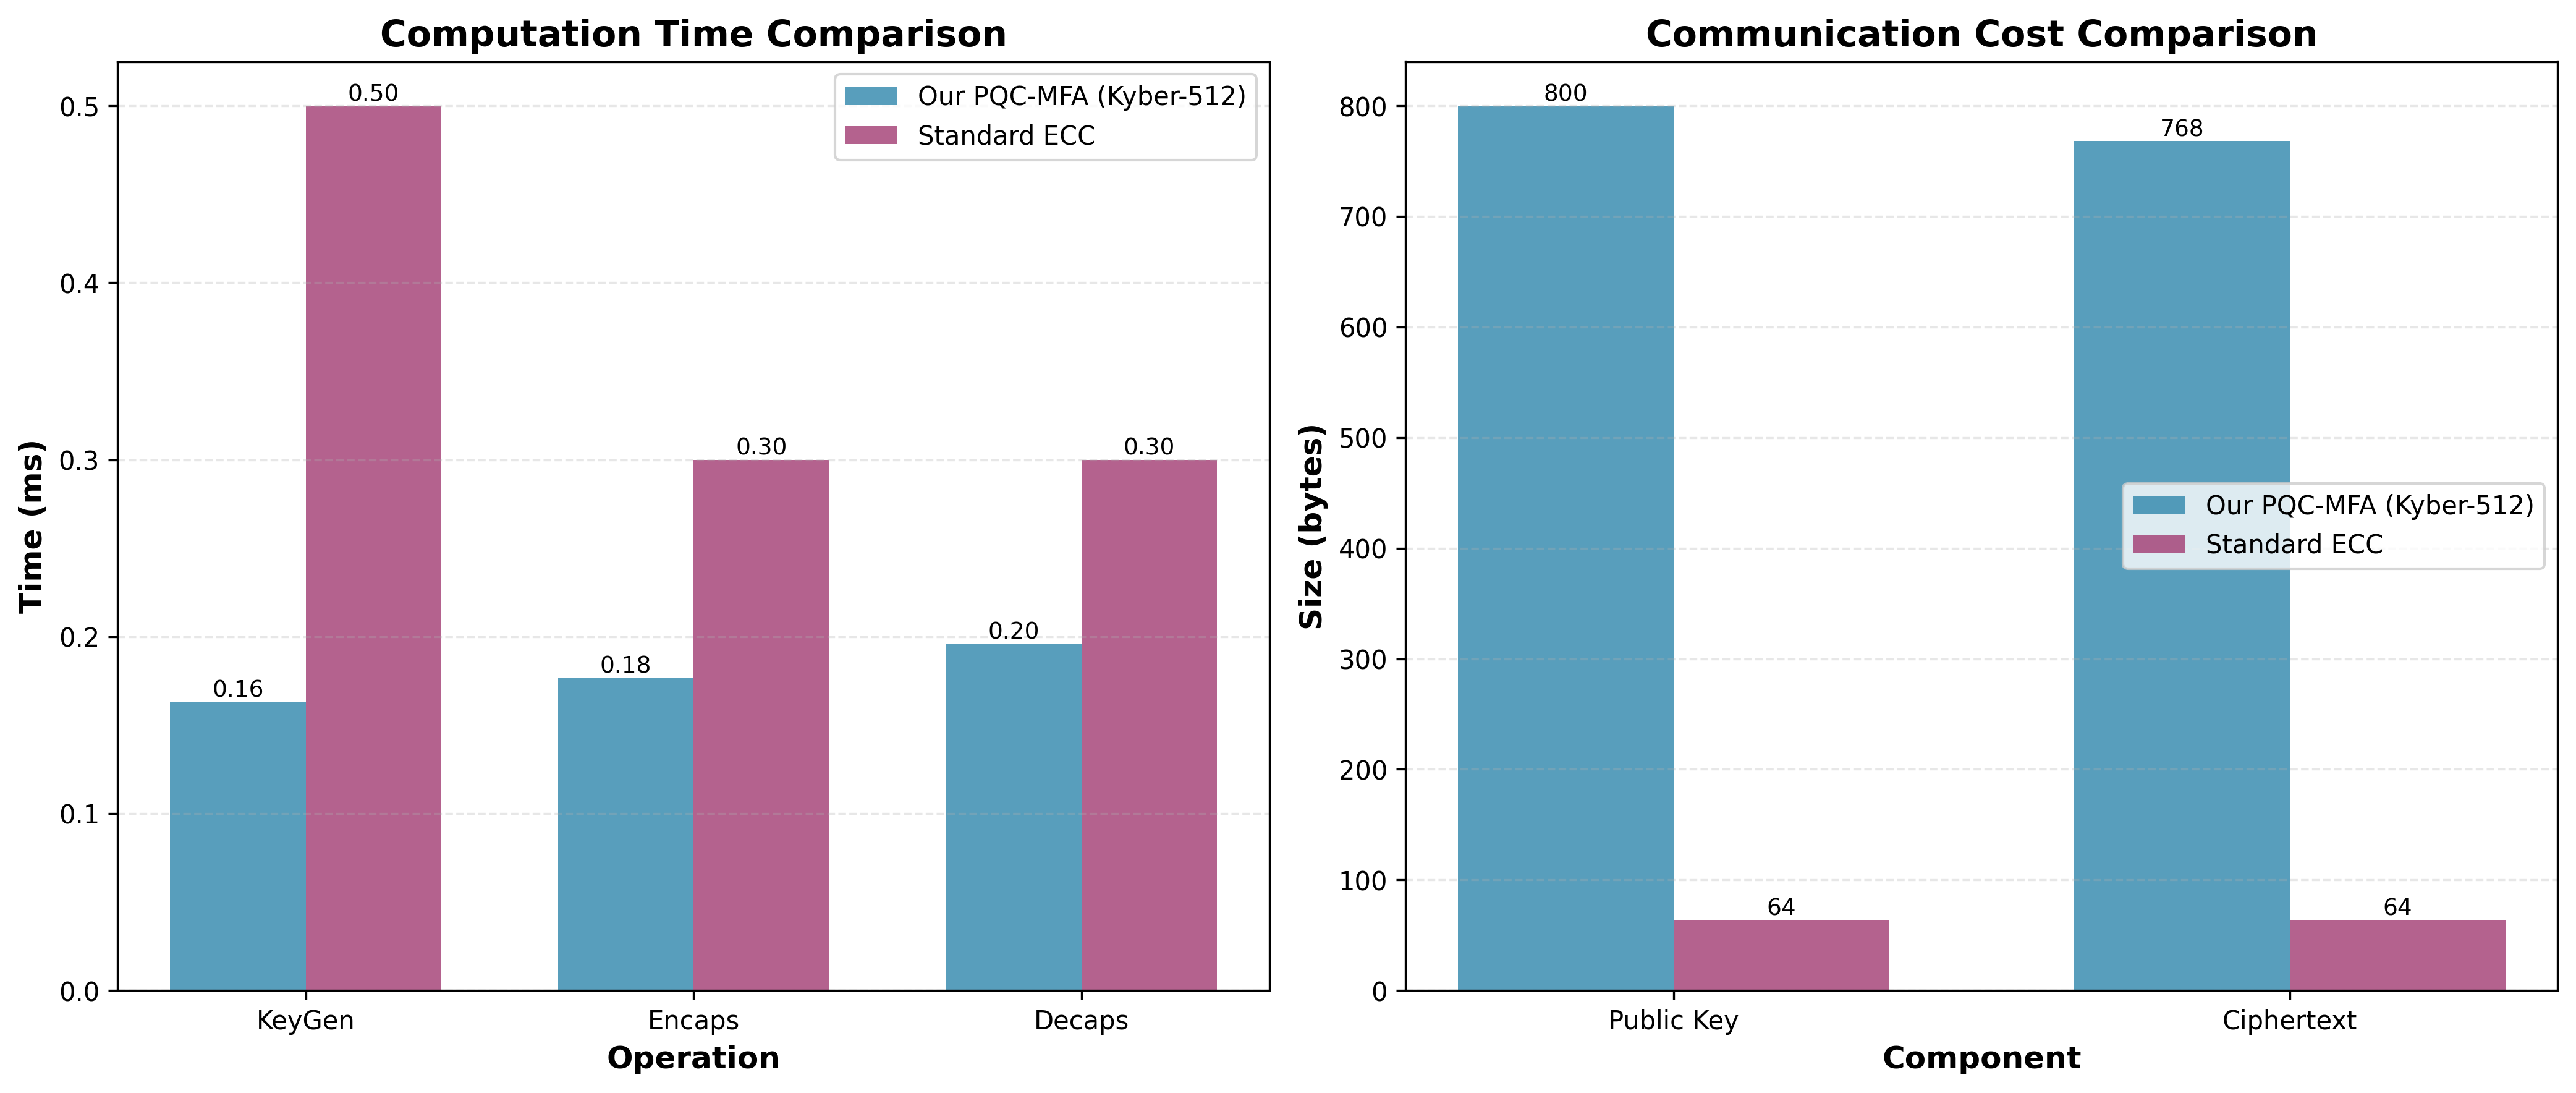
\includegraphics[width=0.8\textwidth]{pqc_mfa_performance_comparison.png}
\caption{Performance Comparison: PQC-MFA (Kyber-512) vs Standard ECC}
\label{fig:performance}
\end{figure}

\section{Formal Verification Results}

\begin{figure}[h]
\centering
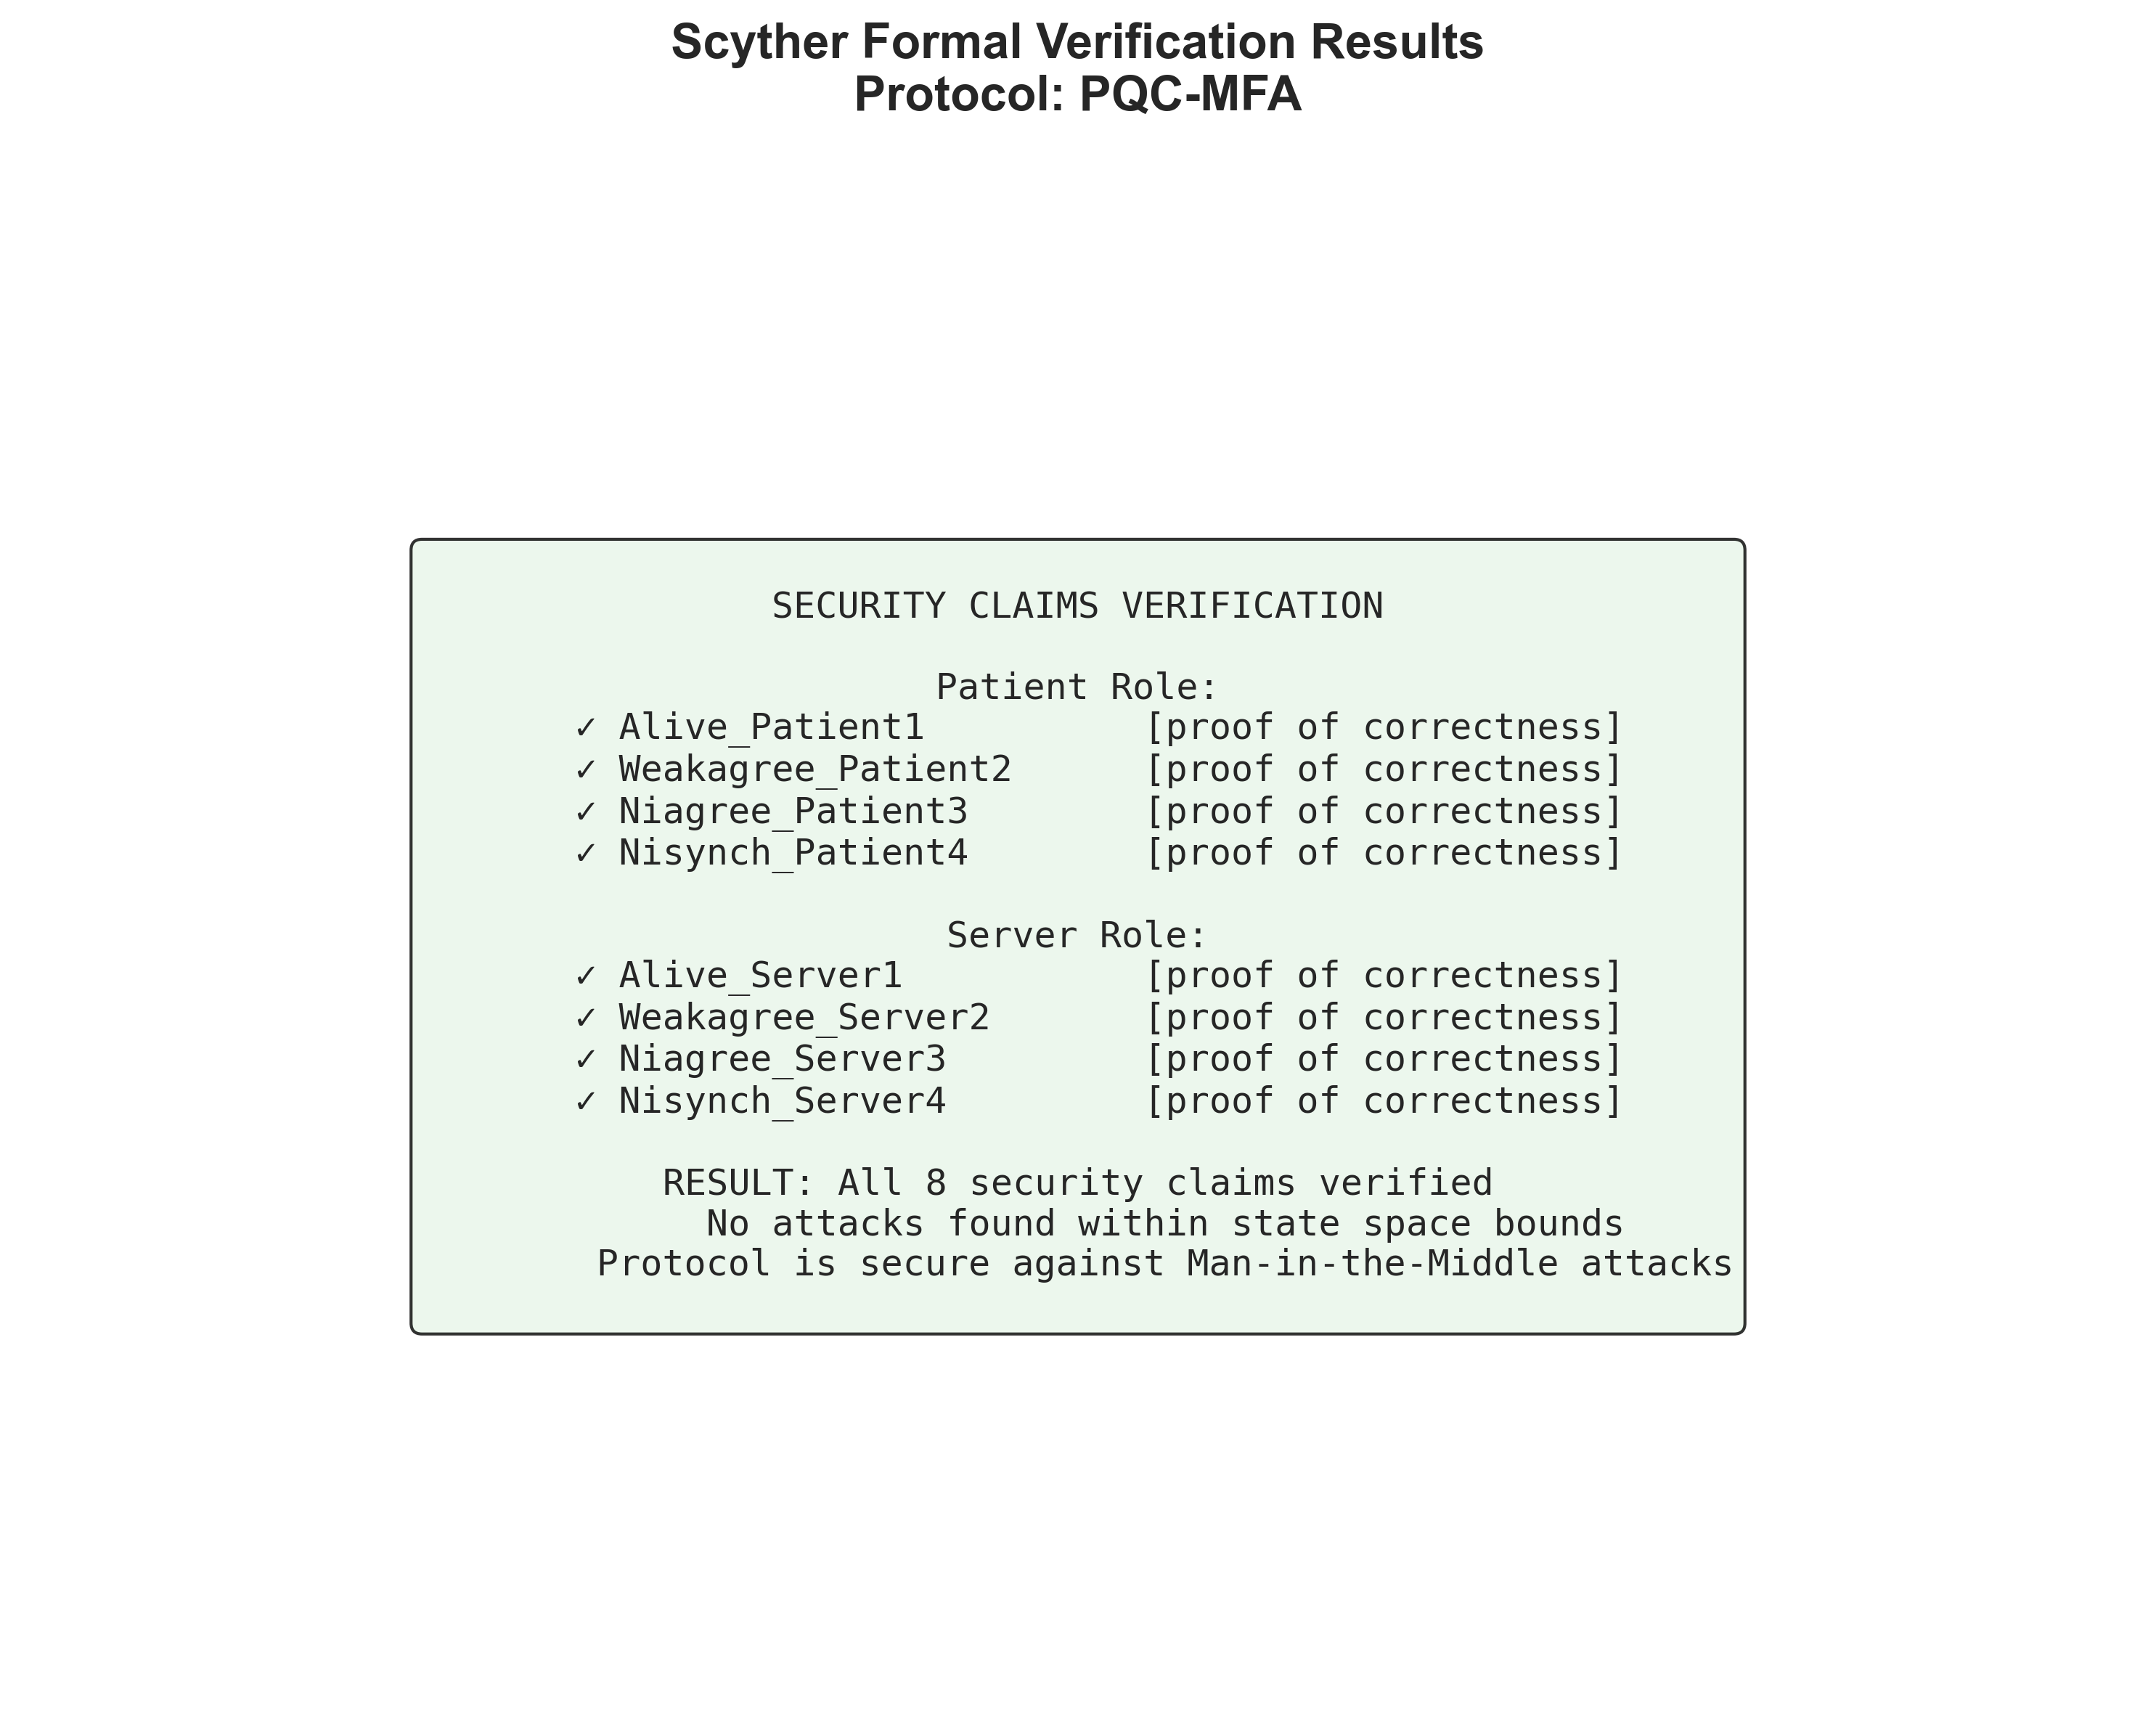
\includegraphics[width=0.8\textwidth]{scyther_verification_results.png}
\caption{Scyther Formal Verification Results}
\label{fig:scyther}
\end{figure}

\section{Conclusion}
Your conclusion text here.

\end{document}
